\chapter{Nueva funcionalidad}
\label{ch:news}
Se detalla en las siguientes secciones la nueva funcionalidad agregada (no incluye el manejo de los datos en \textsc{DataPicker} ya que se describe como parte del refactoring), con la que se pretende implementar la funcionalidad en l\'inea de  este programa. 

\section{Manejo de la rutina: \textsc{RoutineHandler}}

La \textbf{rutina} se entiende como la ejecuci\'on completa del programa, con la cual se procesan todas las observaciones de acuerdo a una lista de CCDs y campos. Para esta finalidad se cre\'o una clase llamada \textsc{RoutineHandler} la cual maneja los archivos de entrada de:

\begin{itemize}
\item Lista de campos, CCDs y semestres en un archivo CSV (en este mismo orden) y con el encabezado \texttt{Field, CCD, Semester}.  
\item Diccionario de directorios y expresiones regulares de las ubicaciones de los archivos y sus nombres, respectivamente (archivo TXT). 
\item Diccionario de umbrales y valores relevantes en la ejecuci\'on del programa, as\'i como el tipo de filtro a usar (archivo TXT).
\end{itemize}
\bigskip

El diccionario de umbrales y valores de configuraci\'on contiene la siguiente lista de valores:

\begin{itemize}
\item \texttt{imgHeight}: Altura de las im\'agenes cient\'ificas.
\item \texttt{imgWidth}: Ancho de las im\'agenes cient\'ificas.
\item \texttt{filter}: Tipo de filtro (\texttt{basic}, \texttt{mcc} o \texttt{ukf}).
\item \texttt{results}: Directorio de resultados (donde guardar estos).
\item \texttt{init\_var}: Varianza inicial que tendran las matrices de covarianza durante el proceso de estimaci\'on con los filtros de Kalman. 
\item \texttt{flux\_thresh}: Umbral del estado de flujo obtenido con Kalman. 
\item \texttt{flux\_rate\_thresh}: Umbral de la velocidad de flujo obtenido con Kalman.
\item \texttt{rate\_satu}: Tasa de saturaci\'on 
\item \texttt{sigma\_a}: Varianza para Kalman B\a'sico.
\item \texttt{epsilon}: Radio de error con que la estimaci\'on por filtro de Kalman de m\'axima correntrop\'ia disminuye la ganancia de Kalman. Corresponde a un criterio de detenci\'on.
\item \texttt{max\_iter}: N\'umero de iteraciones m\'aximo para el proceso de correcci\'on al usar Kalman de m\'axima correntrop\'ia. 
\item \texttt{silverman}: \textit{Entero} toma valor 1 en caso de considerarse, y 0 si no. Se establece si se usa o no la aproximaci\'on de Silverman para determinar ancho de banda del kernel al emplear el filtro de m\'axima correntrop\'ia.
\item \texttt{std\_factor}: Factor de incremento de sigma al usar el m\'etodo de Silverman.
\item \texttt{sigma}: Sigma usado por defecto, sin Silverman, en la determinaci\'on del kernel durante el proceso de correcci\'on con el Filtro de Kalman de m\'axima correntrop\'ia.
\end{itemize}


Esta clase contiene los siguientes m\'etodos:
\begin{itemize}
\item \texttt{process\_settings():}\\
En este m\'etodo se lee el archivo de diccionario de umbrales y valores con los que se configurar\'a la toma de decisiones del programa.
\bigskip

\item \texttt{retrieve\_kalman\_filter(kalman\_string):}\\
Corresponde a un m\'etodo auxiliar que es invocado desde \texttt{process\_settings} con el que se crea una instancia del filtro de Kalman a partir de la lectura del archivo de valores, de acuerdo al valor defindo por el usuario. Los tres strings v\'alidos para la construcci\'on de una instancia son: 'Basic', 'MCC' y 'UKF'. Si se entrega otro tipo de string, se levanta un error.
\bigskip
  
\item \texttt{iterate\_over\_sequences():}\\
Recorre la lista de campos, CCDs y semestres entregada al programa con la consiguiente llamada a \texttt{routine}
\bigskip

\item \texttt{routine(semester, field, ccd, results\_path, last\_mjd):}\\
Corresponde a la rutina que comprende el an\'alisis de las observaciones de un semestre, campo y CCD espec\'ifico. 
\end{itemize}  
\bigskip

\section{Detecci\'on de fen\'omenos transitorios: \textbf{TPDetector}}
Es una peque\~na clase con la que se apoya el proceso de reconocimiento o detecci\'on de alg\'un fen\'omeno transitorio en el comportamiento de la intensidad de los pixeles calculados despu\'es la ejecuci\'on de \texttt{routine} (es decir, una vez que se han obtenido los resultados con \texttt{routine} de \textsc{RoutineHandler}).
\bigskip

Esta clase posee los siguientes m\'etodos:

\begin{itemize}
\item \texttt{look\_candidates(results\_path, field, ccd, semester)}:\\
Con este m\'etodo se agrupan los resultados obtenidos por campo, CCD y semestre en la ruta de los resultados (\texttt{results\_path}), y carga los arreglos de los candidatos encontrados (de acuerdo a su coordenada central) y cuenta las veces que aparece cada uno en los archivos (un archivo por \'epoca u observaci\'on) con la finalidad de registrar \textit{las veces que ha sido candidato}.  
\bigskip

\item \texttt{list\_candidates(cand\_mid\_coords)}\\
Con finalidades exploratorias, este m\'etodo registra los candidatos (por pares de pixeles que describen el centro de los grupos encontrados) sin repetici\'on, independiente de las veces que han aparecido.
\end{itemize}

  
\section{\textsc{DataContent}}
\textsc{DataContent} es una clase auxiliar que es usada principalmente para encapsular los resultados obtenidos durante el proceso de detecci\'on, tanto de los pixeles de los grupos encontrados por \'epoca, la lista de pixeles centrales de estos grupos, las matrices de etiquetas (para realizar seguimiento de las causas del descarte de los pixeles o grupo de pixeles), as\'i como tambi\'en los estados encontrados por el filtro usado. Para guardar estos resultados se utiliza la funci\'on \texttt{savez} de la librer\'ia \textsc{Numpy}, los archivos guardados son registrados en un archivo de extensi\'on NPZ.
\bigskip

Para el guardado de los datos se implement\'o la funci\'on \texttt{save\_results} que recibe como par\'ametros la ruta donde se quiere almacenar los resultados, el campo de observaci\'on, el CCD, el MJD y la matriz de estados junto con la covarianza de estados. El resto de los arreglos son definidos en las funciones \texttt{set\_mid\_coords} y \texttt{group\_info}.
\bigskip

La figura \ref{fig:new_routine} muestra diagrama de flujo del programa refactorizado. Desde el script \texttt{exec} se declara una instancia de \textsc{RoutineHandler}, desde la cual se calculan los flujos y se crea una instancia de un filtro de Kalman (alg\'un objeto de la familia \textsc{KalmanFilter}). Posteriormente, el m\'etodo \texttt{draw\_complaying\_pixel\_groups} de un objeto de la clase \textsc{SourceFinder} agrupa y filtra los pixeles y grupos de pixeles que pudiesen ser parte de alg\'un candidato. Finalmente los datos de estos candidatos son guardados con el m\'etodo \texttt{save\_results}. Estos pasos se repiten a medida que hayan \'epocas (observaciones) de que no se hayan procesado.    

\begin{figure}
\centering
\includegraphics[scale=.5]{/home/paloma/Documents/Memoria/Code/sif2/sif2_act}
\label{fig:new_routine}
\caption{Rutina del programa refactorizado.}
\end{figure}


\section{Nuevo m\'etodo en Visualizer}

Se implement\'o una nueva funci\'on con la que visualizar el espacio de fase del flujo y su velocidad estimada.

\texttt{print\_space\_states(coords, position, save\_filename)}\\

Esta funci\'on recibe como entradas la coordenada del objeto, la posici\'on en estampillas determinadas anteriormente (para no cargar todas las matrices de estado y covarianza en memoria) y un nombre de archivo en \texttt{file\_name}. La Figura \ref{fig:sp_st} muestra un ejemplo de gr\'afica generada del espacio de estado.  

\begin{figure}
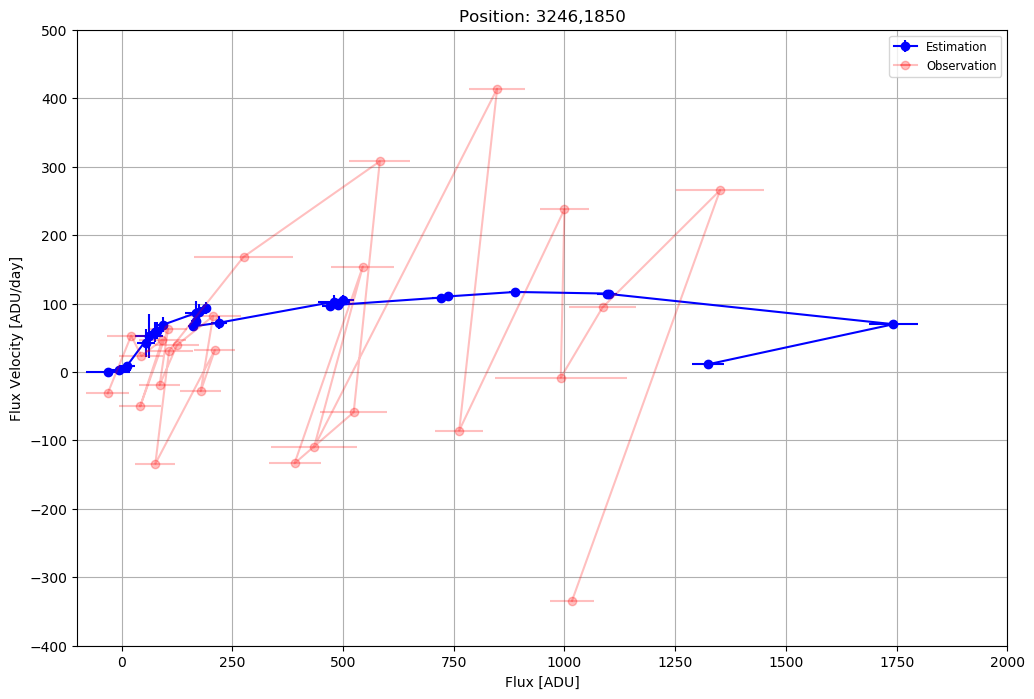
\includegraphics[scale=.5]{images/space_curve.png}
\caption{Espacio de fase de flujo y velocidad de flujo. En azul se destaca la estimaci\'on lograda por filtro de Kalman. En rojo, corresponde al comportamiento del flujo observado y su varianza. Se destaca la vuelta que da la curva azul antes de los 1750 ADU estimados ya que esta da cuenta el alcance m\'aximo en la curva de la supernova y su pr\'oximo decaimiento.}
\label{fig:sp_st}
\end{figure}

\section{\textsc{Filtro de Kalman Unscented}}
El dise\~no de la nueva clase de filtro se realiz\'o continuando con la arquitectura del patr\'on Strategy, definiendo los m\'etodos de predicc\'on y correcci\'on en instancias de clases que implementen las interfaces \textsc{IPredict} e \textsc{ICorrect} respectivamente: \textsc{UnscentPredict} y \textsc{UnscentCorrect}.

\subsection{La clase \textsc{UnscentKalman}}

El filtro Unscented se desarroll\'o en la clase \textsc{UnscentKalman}, la cual encierra los m\'etodos de predicci\'on y correcci\'on (descritos en el Cap\'itulo \ref{ch:background}, subsecci\'on \ref{ssec:ukf}) implementados en \texttt{predict} y \texttt{correct}.
\bigskip

La generaci\'on de una instancia de esta clase requiere como argumentos de entrada los siguientes par\'ametros:

\begin{itemize}
\item \texttt{f\_func:} Funci\'on usada para obtener el primer conjunto de puntos sigma para el periodo de predicci\'on. Consiste en una funci\'on vectorial que se aplica sobre cada elemento de una matriz cuya dimensi\'on es la misma que la de la matriz de estado.
\item \texttt{h\_func:} Funci\'on usada para obtener el segundo conjunto de puntos sigma durante el proceso de correcci\'on. Su aplicaci\'on procede de la misma forma que la descrita para \texttt{f\_func}. 
\item \texttt{alpha:} T\'ermino que indica que tan separados se encuentran los puntos sigma en torno a la media. Por lo general su valor oscila entre $10^{-4}$ y $1$. 
\item \texttt{beta:} Describe el valor de $beta$ el cual incorpora conocimiento \textit{a priori} sobre la distribuci\'on de las variables de estado. Para distribuciones gaussianas, tiene un valor de $\beta=2$. 
\item \texttt{kappa:} Corresponde a un par\'ametro de escalamiento secundario. Su valor va entre $0$ y $3-N$.
\item \texttt{image\_size:} Dimensiones de la imagen de flujo.
\end{itemize}

Al inicializar una instancia de esta clase, se calculan tanto los pesos como el t\'ermino $lambda$, los cuales dependen de los par\'ametros: $\beta$, $\kappa$ $\alpha$ y N o cantidad de variables de estado (ver Ecuaciones \ref{eq:eq20} y \ref{eq:eq21}).
\bigskip

Como parte de la familia de \textsc{KalmanFilter} posee el m\'etodo \texttt{update}, desde el cual se llama a \texttt{predict} y a \texttt{correct}, conservando la firma.
 
\subsection{Predicci\'on}
La predicci\'on de este filtro se implement\'o, como se mencion\'o anteriormente, en la clase \textsc{UnscentPredict} (que implementa \textsc{IPredict}). Para instanciar esta clase se debe entregar como argumento al constructor: un puntero a funci\'on (que puede o no ser lineal), los pesos asociados a la media y la covarianza de predicci\'on, el coeficiente $\lambda$, y la dimensi\'on de las variables de estados (en este modelo, se trata de dos: flujo y velocidad de 
flujo). Por lo tanto la firma del constructor queda como sigue:
\bigskip
\begin{center}
\texttt{UnscentPredict(f\_func, Wm, Wc, lambda\_, N)}
\end{center}
\bigskip

donde \texttt{f\_func} corresponde a la funci\'on con la cual se quiere modelar el comportamiento del flujo; \texttt{Wm} y \texttt{Wc}  corresponden a los pesos de la media y covarianza respectivamente (obtenidos externamente), \texttt{lambda\_} y \texttt{N} correspondiente al n\'umero de variables de estado.
\bigskip

Se destaca que tantos los pesos como el valor de $\lambda$ se mantienen constantes durante todo el proceso de estimaci\'on. Por otro lado, en el mismo m\'etodo, se calculan los \textit{puntos sigma} (ver Ecuaci\'on \ref{eq:eq18}) los cuales, para su determinaci\'on requieren los pesos y del valor de $\lambda$, adem\'as de la funci\'on  $f$ (entregada como \texttt{f\_func}) para evaluar en los puntos sigma.
\bigskip

La salida de este m\'etodo est\'a compuesta por la matriz de estado predicha, la predicci\'on de la covarianza y los puntos sigma guardados en la variable \texttt{Xs} de la implementaci\'on.

\subsection{Correcci\'on}
El proceso de correcci\'on est\'a implementado en la clase \textsc{UnscentCorrect} la cual implementa la interfaz \textsc{ICorrect} redefiniendo el m\'etodo \texttt{correct}. Al venir de la misma familia, este m\'etodo conserva siempre su firma. 
\bigskip

Durante la correcci\'on se escogen nuevamente $2N+1$ puntos sigma en torno al estado predicho (fase previa) (ver Ecuaci\'on \ref{eq:eq24}), sin embargo los valores de los pesos y de $\lambda$ son los mismos usados durante la fase de predicc\'on, cambiando s\'olo la funci\'on que se propaga sobre este nuevo conjunto de puntos: $h(\dot)$ (expresada como \texttt{h\_func}). 
\bigskip

\subsection{Funciones auxiliares}
Se desarrollaron diferentes funciones auxiliares para apoyar el c\'alculo de las matrices:
\begin{itemize}
\item \texttt{sigma\_points(mean\_, cov\_, lambda\_, N):}\\
Funci\'on con la cual se calculan los puntos sigma a partir la media de las variables de estado, la covarianza, el valor de $\lambda$ y el n\'umero de variables de estado, N. Utiliza para esta finalidad, la descomposici\'on de Cholesky.
\item \texttt{unscent\_weights(kappa, alpha, beta, N):}\\
M\'etodo con el que se calculan los pesos a partir de los valores de $\kappa$, $\alpha$, $\beta$ y N (n\'umero de variables de estado). 
\item \texttt{perform(func, *args):}\\
Funci\'on auxiliar con la cual se recibe un puntero a otra funci\'on vectorial (destinada a ser aplicada sobre un conjunto de puntos sigma) y un n\'umero arbitrario de argumentos, dependiendo de la necesidad de la misma funci\'on
\item \texttt{propagate\_func(func, Wm, Wc, Xs, *args, N):}\\
Funci\'on con la que se propaga la funci\'on \texttt{func} sobre el conjunto de puntos sigma \texttt{Xs} usando los pesos de media y covarianza \texttt{Wm} y \texttt{Wc}, respectivamente, adem\'as del n\'umero de variables de estado, N. Adem\'as, recibe el argumento \texttt{args} que corresponde a una tupla de entradas propias de la funci\'on \texttt{func}.  
\item \texttt{matrix\_inverse(M):}\\
Calcula la inversa de una matriz siguiendo la estructura de datos descrita en el Cap\'itulo \ref{ch:prev_work}.
\item \texttt{matrix\_vector\_dot\_product(M, v):}\\
Funci\'on auxiliar para el c\'alculo del producto punto entre una matriz (cuya dimensi\'on es la de una matriz de covarianza definida en el Cap\'itulo \ref{ch:prev_work}) y un \textit{vector} de las dimensiones de una matriz de estado (ver mismo cap\'itulo).
\end{itemize}

Estas funciones est\'an implementadas en el script \texttt{unscented\_utils}.
